\documentclass[border=3pt]{standalone}
%\usepackage{amsthm}
\usepackage{amsmath}
\usepackage{amssymb}
\usepackage{natbib}
\usepackage[colorlinks,citecolor=blue,urlcolor=blue,filecolor=blue,backref=page]{hyperref}
\usepackage{graphicx}
\usepackage{subfigure}
\usepackage{bm}
\usepackage{booktabs}
\usepackage{listings}
\usepackage{color}

\usepackage{tikz}
\usetikzlibrary{shapes.misc}
\usetikzlibrary{matrix}
\usetikzlibrary{arrows,backgrounds,fit,calc,shapes,automata}
\usetikzlibrary{bayesnet}
\tikzstyle{every picture}+=[remember picture]
\tikzset{
    %Define standard arrow tip
    >=stealth',
    %Define style for boxes¡
    punkt/.style={
           rectangle,
           rounded corners,
           draw=black,
           thick,
           text width=3.5cm,
           minimum height=1.0cm,
           text centered},
    % Define arrow style
    pil/.style={
           ->,
           thick,
           shorten <=2pt,
           shorten >=2pt,}
}
\usetikzlibrary{decorations.pathreplacing,shapes}
\pagestyle{empty}

\begin{document}
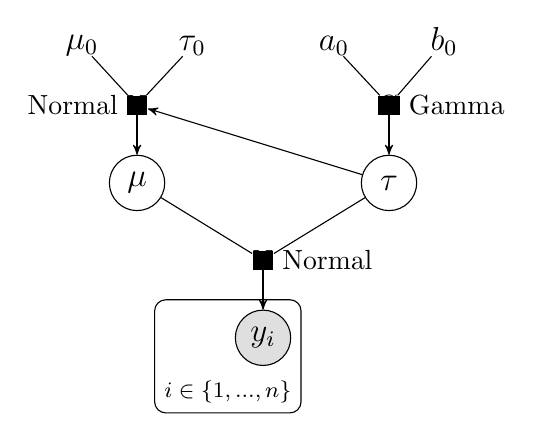
\begin{tikzpicture}[scale=1.0, transform shape]
  [squarednode/.style={rectangle, draw=black, minimum size=8mm},
    latent/.style={circle, draw=black, minimum size=10mm}]

  % \footnotesize

  % Define nodes
  \node[obs]                               (y) {\large $y_i$};

  \node[factor, above=0.5cm of y, xshift=0cm]  (N2) {N};
  % \node[const, right=0.1cm of G] () {\normalsize $\mathcal{G}$};
  \node[const, right=0.1cm of N2] () {\normalsize Normal};


  \node[latent, above=1.25cm of y, xshift=1.6cm]  (tau) {\large $\tau$};
  \node[const, above=1.25cm of tau, xshift=-0.7cm]  (a0) {\large $a_0$};
  \node[const, above=1.25cm of tau, xshift=0.7cm]  (b0) {\large $b_0$};

  \node[factor, above=0.5cm of tau, xshift=0cm]  (G) {G};
  % \node[const, right=0.1cm of G] () {\normalsize $\mathcal{G}$};
  \node[const, right=0.1cm of G] () {\normalsize Gamma};

  \node[latent, above=1.25cm of y, xshift=-1.6cm]  (mu) {\large $\mu$};
  \node[const, above=1.25cm of mu, xshift=-0.7cm]  (mu0) {\large $\mu_0$};
  \node[const, above=1.25cm of mu, xshift=0.7cm]  (tau0) {\large $\tau_0$};

  \node[factor, above=0.5cm of mu, xshift=0cm]  (N) {N};
  % \node[const, right=0.1cm of G] () {\normalsize $\mathcal{G}$};
  \node[const, left=0.1cm of N] () {\normalsize Normal};



  % \draw [->] (tau) -- (y);
  \draw [->] (tau) -- (N);
  % \draw [->] (mu) -- (y);

  \factoredge{a0,b0}{G}{tau}
  \factoredge{mu0,tau0}{N}{mu}
  \factoredge{mu,tau}{N2}{y}

  \plate {} {(y)} {$i \in \{1, ..., n \}$}; %

\end{tikzpicture}
\end{document}
